\section{Ground Loop Computational Results}
%
We can construct a MATLAB program that allows use to simulate different possible scenarios. In doing so we hope to discover key conditions that would make a ground loop system favorable for the buyer. The implementation has ignored the resistance added by the soil. In practice if the designer can calculate how far radially outward the temperature gradient in the soil becomes close to zero the derived formulas can be used. The soil is a infinite medium and thus would have to be solved with a unsteady diffusion formulation. The problem is formulated with a 1" HDPE pipe with a wall thickness of 1/16". The mass flowrate is varied to see how this affects the outlet temperature. The inlet temperature is around 73 degrees and the ground was taken to be 55 degrees which is the average ground temperature in Delaware \cite{SoilTemps}. Using these assumptions the pipe system can be simulated.
%
\begin{figure}[H]
    \centering
    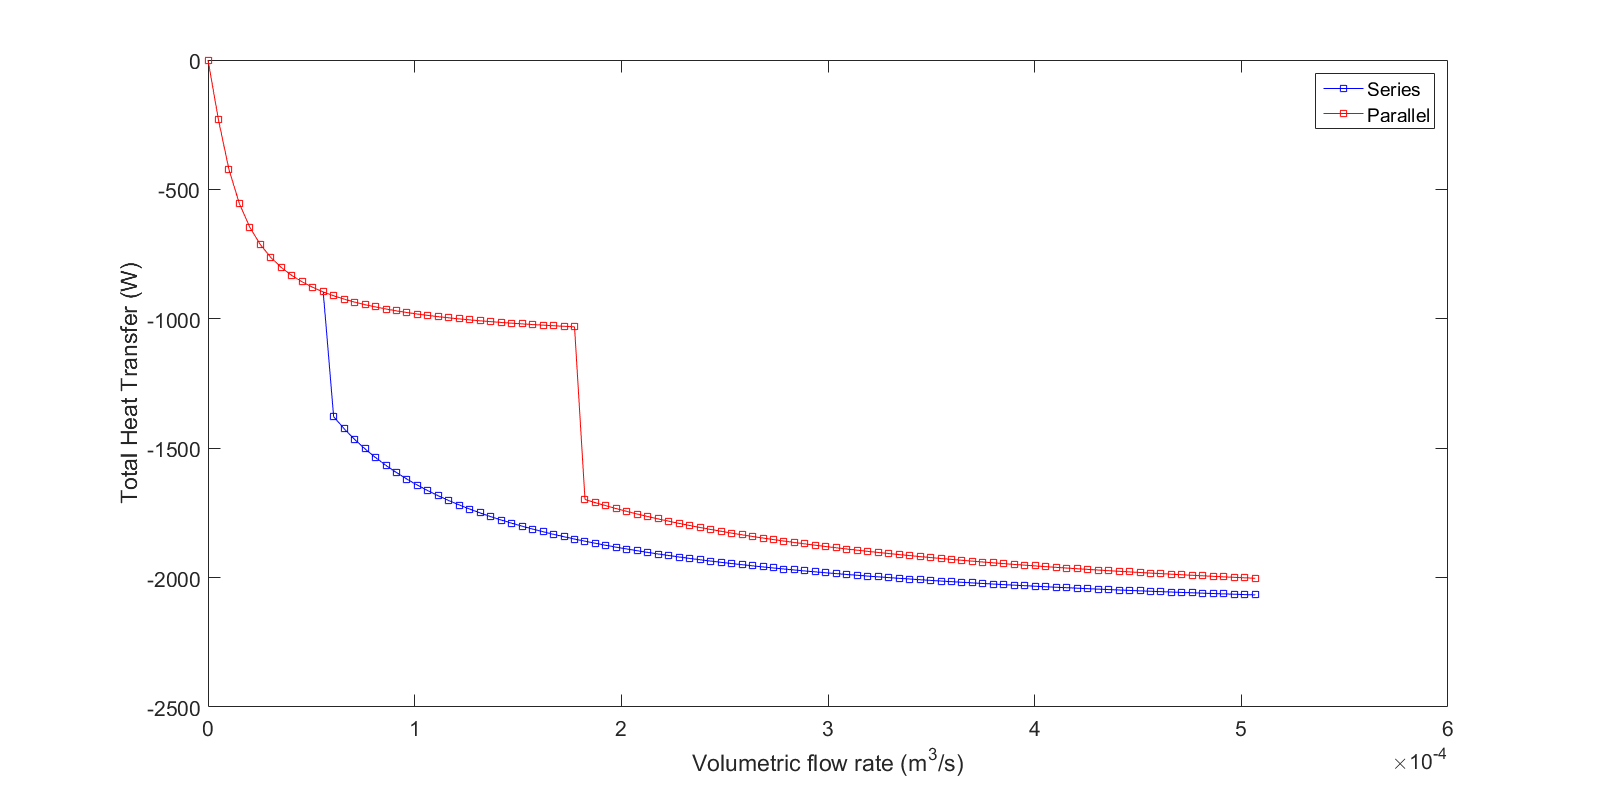
\includegraphics[height=3.5in]{pictures/heat_11_ground_23_inlet.png}
    \caption{Total heat transfer for a 30 meter long pipe with varying flowrate. Parallel uses 3 tubes being of length of 10 meters.}
\end{figure}
%
\begin{figure}[H]
    \centering
    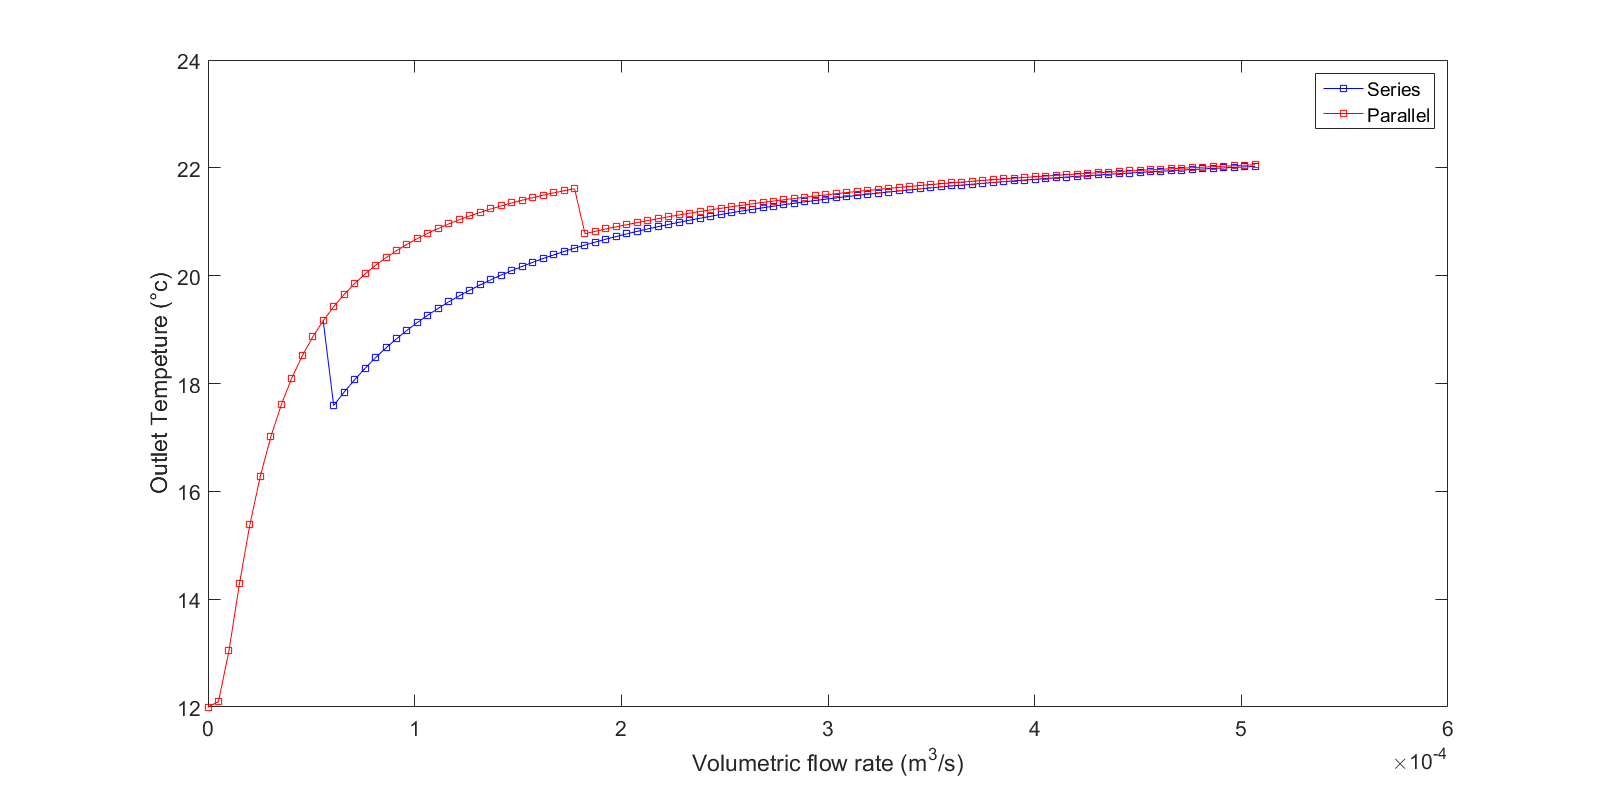
\includegraphics[height=3.5in]{pictures/outlet_11_ground_23_inlet.png}
    \caption{Final outlet temperature for a 30 meter long pipe with varying flowrate. Parallel uses 3 tubes being of length of 10 meters. Note the jumps are from the transition from laminar to turbulence.}
\end{figure}
%
\noindent
As seen above there are some very interesting results. The goal of the water loop system is to cool down the hot water exiting the house. This temperature difference can be used in a heat exchanger attached to the house's vapor compression HVAC system to provide summertime cooling. When selecting a system it can be seen that when a series system the flow transitions to turbulent at a lower \textit{total} mass flowrate and therefor allows for a higher heat extraction compared to the parallel configuration.
%
\begin{figure}[H]
    \centering
    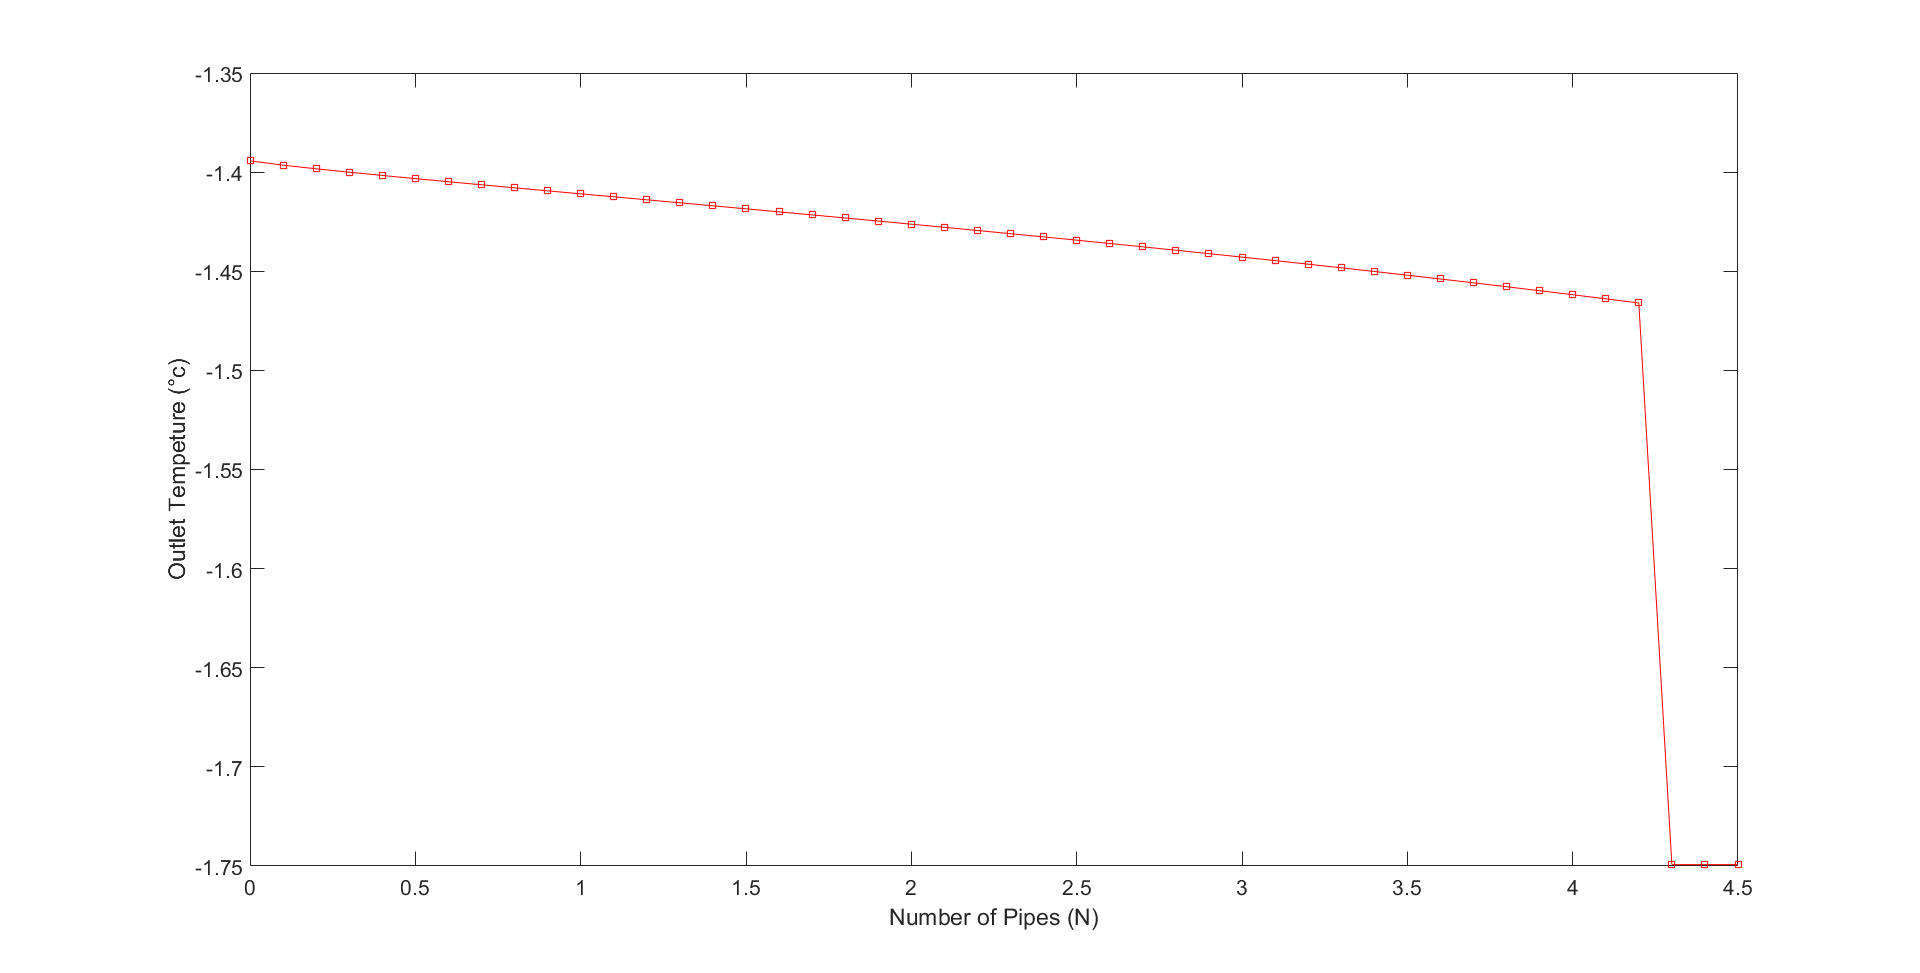
\includegraphics[height=3.5in]{pictures/outlet_parallel_num_pipes.png}
    \caption{Final outlet temperature for a varying number of 30 meter long pipes.}
\end{figure}
%
\noindent
Additionally as seen above as more pipes are added to a parallel system the outlet temperature converges back to the inlet temperature. This is likely because while the total mass flowrate stays constant the flow through each individual pipe decreases and causes a drop in the convection coefficient. The jump seen above shows the transition to laminar flow in all the parallel pipes. A series system has better thermal performance over a parallel system. The downfall to using a series system is that it is likely that a large pump will be needed to reach the same equivalent flowrate of a parallel system. \\ \\
%
In conclusion, a series system allows for higher thermal performance when compared to a parallel system. The parallel system allows for a smaller circulation pump to be used, but has poor heat transfer due to the lower flowrates through the individual pipes in the system. When sizing a system, the total energy needed to be exchanged through the heat exchanger can help select a proper length of tubing.

